\chapter{Redes locais virtuais}\label{chp:vlan}
%%%% https://www.youtube.com/watch?v=H01eZjdcHTo
As redes locais virtuais (\textit{virtual local area networks} -- VLAN) é uma rede local que, embora esteja ligada fisicamente a partir de um mesmo equipamento (\textit{switch}, por exemplo), está segmentada logicamente em duas ou mais redes locais. Cada uma das redes locais lógicas é independente das demais, formando o que chamamos de \enquote{domínio de \textit{broadcast}}. Neste capítulo, vamos ver como configurar uma VLAN usando o \CPT. 

Para ilustrar, vamos supor que em uma instituição exemplo (uma universidade), temos três redes lógicas diferentes, conforme apresentado na \Cref{fig:vlan}. Assim, teremos uma rede lógica para docentes, outra para funcionários e uma terceira para estudantes.

\begin{figure}[!htb]
    \centering
    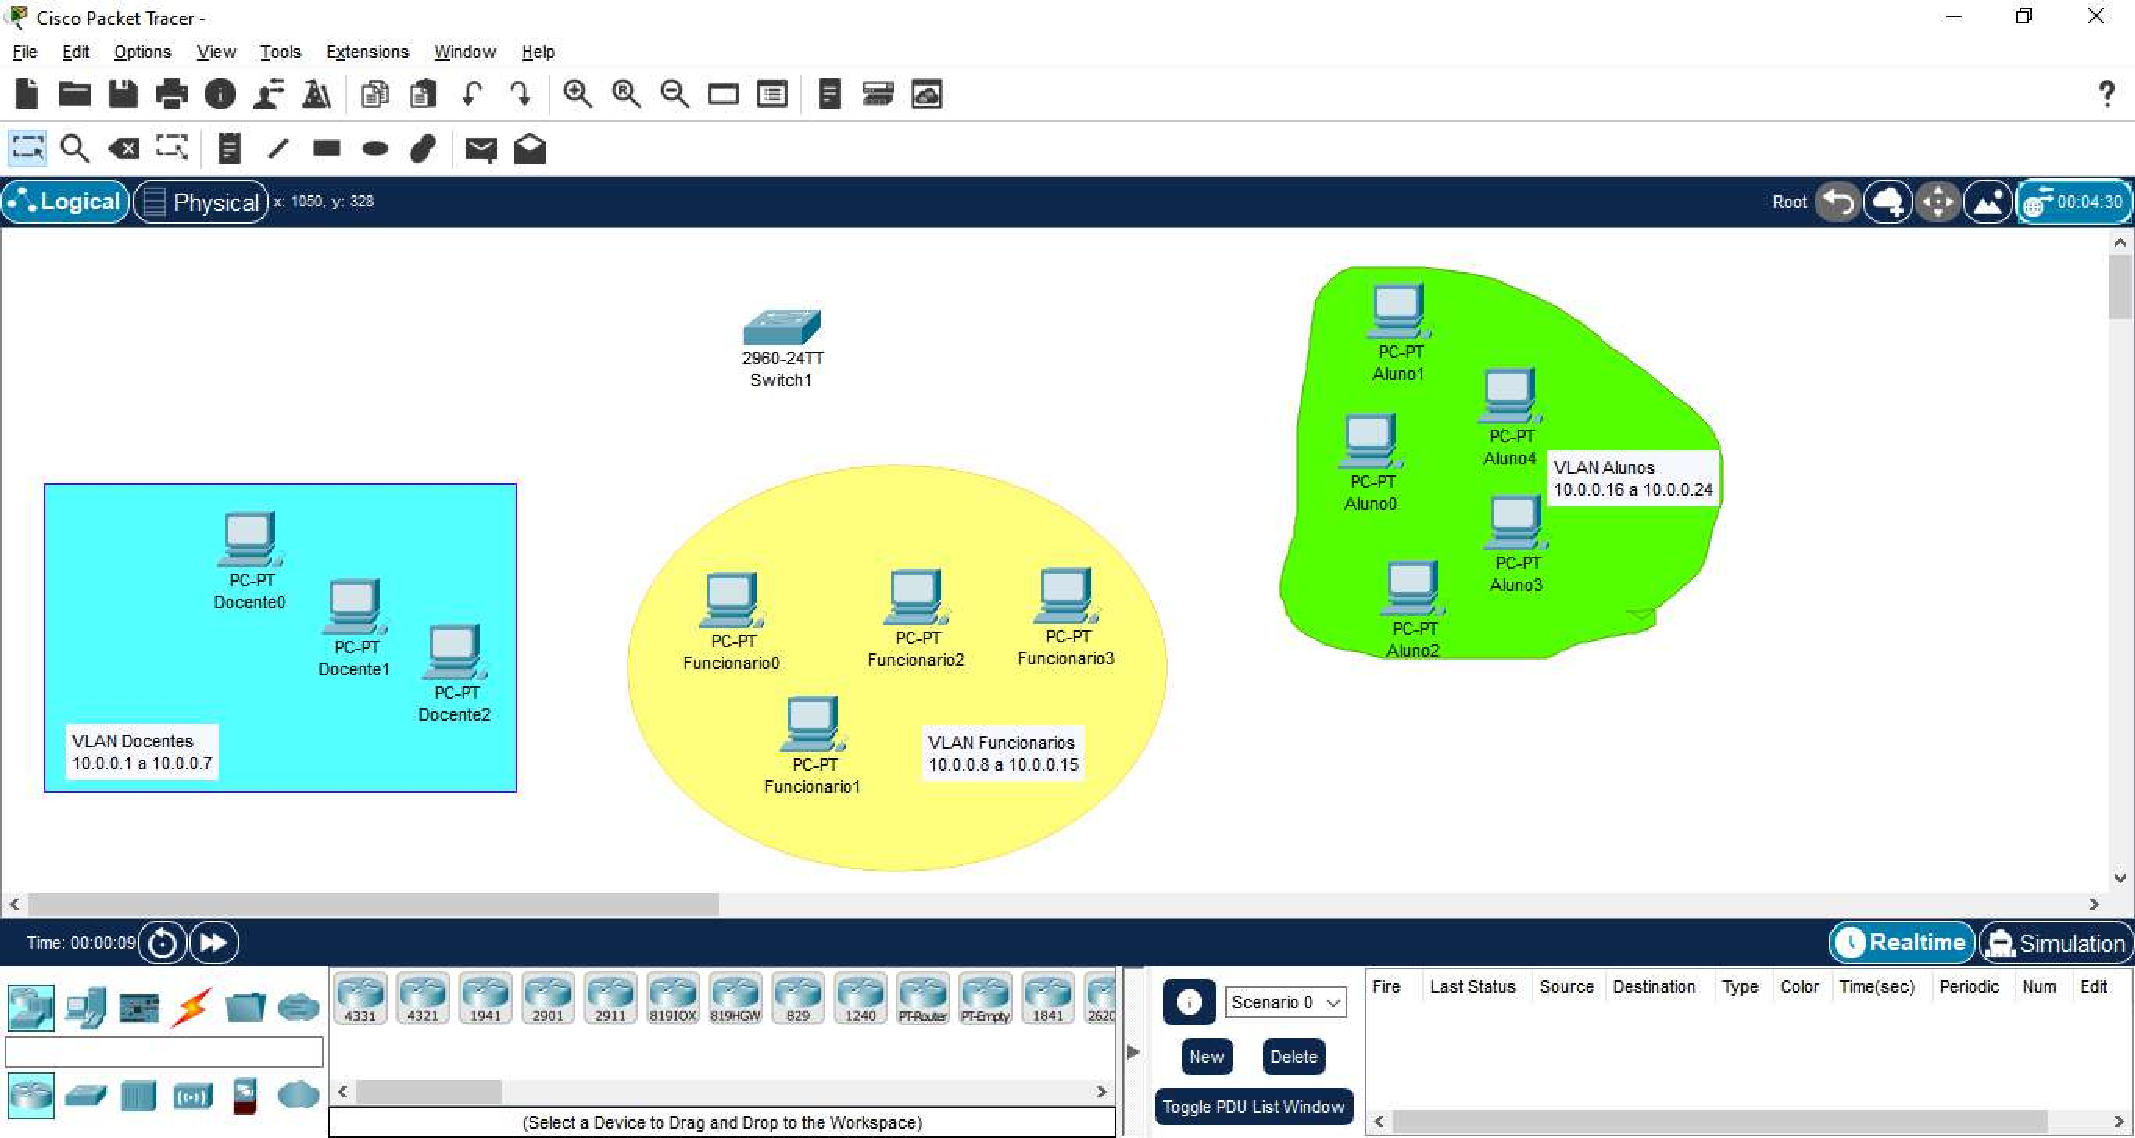
\includegraphics[width=.99\textwidth]{Figuras/vlan}
    \caption{VLANs diferentes em uma organização.}
    \label{fig:vlan}
\end{figure}

\section{Topologia das VLANs}\label{sec:topVLAN}
A topologia proposta para ilustrarmos a configuração de VLANs é a seguinte:
\begin{itemize}
    \item A VLAN para docentes, de início, terá três PCs conectados e terá reservados os endereços IP das faixas \texttt{10.0.0.1} a  \texttt{10.0.0.7}.
    \item A VLAN para funcionários, de início, terá quatro PCs conectados e terá reservados os endereços IP das faixas \texttt{10.0.0.8} a  \texttt{10.0.0.15}.
    \item A VLAN para alunos, de início, terá cinco PCs conectados e terá reservados os endereços IP das faixas \texttt{10.0.0.16} a  \texttt{10.0.0.24}.
\end{itemize}

Note que utilizaremos apenas um \textit{switch} de 24 portas (Modelo 2960) para estabelecer essas VLANs. Perceba também que dividimos oito endereços IPs para cada VLAN, embora não utilizaremos todos em um primeiro momento.

Antes de começar a configuração da VLAN, conecte todos os PCs ao \textit{switch}. \textbf{Atente para a divisão das 
interfaces entre as VLANs}. Dessa forma, faça o seguinte:
\begin{enumerate}[label*=\arabic*.]\label{enum:divInterfaces}
\item Para os PCs da VLAN dos docentes:
   \begin{enumerate}[label*=\arabic*.]
       \item Conecte a interface \texttt{FastEthernet0} do PC \texttt{Docente0} à interface \texttt{FastEthernet0/1} do \textit{switch}.
       \item Conecte a interface \texttt{FastEthernet0} do PC \texttt{Docente1} à interface \texttt{FastEthernet0/2} do \textit{switch}.
       \item Conecte a interface \texttt{FastEthernet0} do PC \texttt{Docente2} à interface \texttt{FastEthernet0/3} do \textit{switch}.
   \end{enumerate}
\item Para os PCs da VLAN dos funcionários:
   \begin{enumerate}[label*=\arabic*.]
       \item Conecte a interface \texttt{FastEthernet0} do PC \texttt{Funcionario0} à interface \texttt{Fast\-Ether\-net0/8} do \textit{switch}.
       \item Conecte a interface \texttt{FastEthernet0} do PC \texttt{Funcionario1} à interface \texttt{Fast\-Ether\-net0/9} do \textit{switch}.
       \item Conecte a interface \texttt{FastEthernet0} do PC \texttt{Funcionario2} à interface \texttt{Fast\-Ether\-net0/10} do \textit{switch}.
       \item Conecte a interface \texttt{FastEthernet0} do PC \texttt{Funcionario3} à interface \texttt{Fast\-Ether\-net0/11} do \textit{switch}.
   \end{enumerate}
\item Para os PCs da VLAN dos alunos:
   \begin{enumerate}[label*=\arabic*.]
       \item Conecte a interface \texttt{FastEthernet0} do PC \texttt{Aluno0} à interface \texttt{FastEthernet0/17} do \textit{switch}.
       \item Conecte a interface \texttt{FastEthernet0} do PC \texttt{Aluno1} à interface \texttt{FastEthernet0/18} do \textit{switch}.
       \item Conecte a interface \texttt{FastEthernet0} do PC \texttt{Aluno2} à interface \texttt{FastEthernet0/19} do \textit{switch}.
       \item Conecte a interface \texttt{FastEthernet0} do PC \texttt{Aluno3} à interface \texttt{FastEthernet0/20} do \textit{switch}.
       \item Conecte a interface \texttt{FastEthernet0} do PC \texttt{Aluno4} à interface \texttt{FastEthernet0/21} do \textit{switch}.
   \end{enumerate}
\end{enumerate}

Aguarde um tempo e verá que todas as comunicações estão funcionando. 

\section{Exercício}
Agora, como teste, verifique se consegue enviar um PDU de um computador da rede \texttt{alunos} para a rede \texttt{docentes}.

Se tudo funcionou bem, perceba que todos os PCs estão em uma mesma rede local. Portanto, todos são acessíveis entre si.

\section{Configuração das VLANs}\label{sec:configVLAN}
Agora vamos configurar cada uma das VLANs. Por uma questão de organização, vamos nomeá-las de \texttt{VLANDocentes}, \texttt{VLANFuncionários} e \texttt{VLANAlunos}, respectivamente.

Toda a configuração será feita no \textit{switch}. Para configurar o \textit{switch}, precisamos acessar a interface da linha de comando (\textit{Command Line Interface} -- CLI). Para isso, clique sobre o \textit{switch} e, depois, selecione a aba \texttt{CLI}.

Ao selecionar a aba \texttt{CLI}, você estará na console de configuração do \textit{switch}. Tecle \keys{\enter} e o \textit{prompt} com a \textit{string} \enquote{\texttt{Switch>}} mostrará que está pronto para receber os comandos. Agora execute os passos a seguir.

\begin{enumerate}[label*=\arabic*.]
    \item Digite \semaspas{enable} para entrar no modo administrador. Note que o \textit{prompt} mudou para \enquote{\texttt{Switch\#}}.
    \item Digite \semaspas{configure terminal} para entrar na configuração global\footnote{Você também pode digitar apenas as primeiras letras do comando. Por exemplo, você poderá digitar apenas \semaspas{conf term} para entrar na configuração global.}. Note que o \textit{prompt} mudou para \enquote{\texttt{Switch (config)\#}}.
    \item Agora defina o número (inteiro) da VLAN que você vai criar. Lembre-se que a \texttt{VLAN 1} é a VLAN \textit{default}. Portanto, as demais VLANs devem começar a partir de \texttt{2}. Assim, para cada VLAN, começando da VLAN 2, vamos executar os passos a seguir:
    
    \begin{enumerate}[label*=\arabic*.]
        \item Digite \semaspas{VLAN X} para entrar na configuração da VLAN X, onde X pode ser 2 (para a rede de docentes), 3 (para a rede de funcionários) ou 4 (para a rede de alunos).
        \item Note que o \textit{prompt} mudou para  \enquote{\texttt{Switch (config-vlan)\#}}. Agora digite o comando a seguir  para atribuir um nome à VLAN que você está configurando. Não esqueça de substituir \texttt{nome\_da\_vlan} pelo nome da respectiva VLAN que você está configurando (\texttt{VLANDocentes}, \texttt{VLANFuncionários} ou \texttt{VLANAlunos}).

        \texttt{\textcolor{green}{Switch(config-vlan)\#} \textcolor{blue}{name} nome\_da\_vlan}

        \item Digite \semaspas{exit} para encerrar a configuração dessa VLAN.
    \end{enumerate}

    \item Depois de terminar todas as configurações de VLANs, digite \semaspas{exit} para encerrá-las.
    
    \item Verifique que todas as VLANs foram criadas com o comando a seguir:  

       \texttt{\textcolor{green}{Switch\#} \textcolor{blue}{show} vlan brief}

    Note que as VLANS já existem, mas ainda não há  interfaces (portas) atribuídas a elas.
       
    \item Agora, vamos atribuir as respectivas portas para cada VLAN. Primeiro, digite \semaspas{conf term} para entrar na configuração global.

    \item Para cada interface, vamos executar os passos a seguir. Lembre-se da divisão das interfaces que fizemos na \Cpageref{enum:divInterfaces}.

       \begin{enumerate}[label*=\arabic*.]
          \item Digite o comando \semaspas{int F0/Y}, substituindo o \texttt{Y} pelo número da interface que você quer configurar.
          \item Digite o comando \semaspas{switchport access VLAN X}, substituindo o \texttt{X} pelo número da VLAN à qual você quer atribuir aquela interface. 
          
          É importante lembrar que, ao pressionar a tecla \keys{\arrowkey{^}} (seta para cima), a CLI repete o último comando.
       \end{enumerate}
    
    \item Depois de configuradas todas as interfaces, digite \semaspas{end} para sair. Ou, se preferir, digite \keys{\ctrl+z} para voltar à raiz do CLI.

    \item Use o comando \semaspas{show vlan brief} para verificar se a distribuição das portas (interfaces) às respectivas VLANs está ok.

    \item Agora digite o comando \semaspas{write} para gravar as alterações. 
\end{enumerate}

\section{Exercício}
Agora, como teste, verifique se as os PCs dentro de uma VLAN são acessíveis entre si. Envie um PDU de um PC em uma VLAN para outro PC na mesma VLAN.

Depois, verifique se você consegue enviar um PDU de um PC em uma VLAN para outro PC em outra VLAN.